\chapter{Feedback Control Design}
\label{chp:controller}

\section{Balancing Controller}
% WHAT you are going to present in this chapter/section
% WHY you are presenting it, and
% HOW you are going to present it

Provided the robotic gymnast is within the region of controllability, a balancing controller is required to bring the system to the unstable equilibrium position. The design approach is based on the premises that the swing-up controller will swing the robotic gymnast within the region of controllability where the balancing controller will steer the robotic gymnast to balancing.

%The balancing of the gymnast will be achieved by catching the gymnast when the swing-up control algorithm has brought the gymnast to the null controllability region. The null controllability region is the set of states that can be steered to inverted unstable equilibrium position in a fixed time with a constrained control input \cite{null_controllability}.
The independent parameters, $\phi$ and $\theta$, will be condensed from now on as a vector describes as $$ \vec{q} = 
\begin{bmatrix}
\theta \\
\phi
\end{bmatrix}
$$

The system can be approximated as a linear system when in the vicinity of the unstable equilibrium position. The system is thus linearised at $$\vec{Q_{s}} = [\vec{q_{s}},\dot{\vec{q_{s}}},\ddot{\vec{q_{s}}}]^{T}=[\pi,0,0,0,0,0]$$ the unstable equilibrium position using the Taylor Series Expansion shown in detail in Appendix B. This linearised model can than be written in the state space form to implement a feedback gain. The state space variables are chosen as $\Delta{\vec{q}}$ and $\Delta{\dot{\vec{q}}}$ which results in the state space representation as:  $$ \dot{\vec{q}} = \boldsymbol{A}\Delta{\vec{q}} + \boldsymbol{B}u $$ and $$ \vec{y} = \boldsymbol{D}\Delta{\vec{q}} + \boldsymbol{0}u $$.

The linearised system remains a coupled system which results that the quadratic eigenvalue problem is required to be solved to identified the poles of the system. The solved quadratic eigenvalue problem results in the following poles from the system parameters in Table \ref{table:system_param}.
$$
\vec{s} = 
\begin{bmatrix}
-8.2 \\
-4.2	\\
8.2 \\
4.2 \\

\end{bmatrix}
$$

The poles of the system are pairs of positive and negative real poles that indicates an unstable system. This is expected due to the system being linearised in the unstable equilibrium position. When the linearised system is at rest, any disturbance will result in a theoretically infinite growth of the state variables, but this behaviour can be controlled by introducing feedback. \\
\\
These poles will be moved to the desired position by using the method of dominant poles. The method of dominate poles chooses a pair of the poles for the closed-loop system and select the other open-loop poles to have real parts. This allows the higher-order system response to be characterised as a second-order response \cite{textbook}. The linearised model already has 2 negative real poles which is chosen to stay the same. The real positive poles were selected based on the following specifications.

These specification was selected on increasing the null controllability region with a low settling time. Due the approximation of the linearised model the null controllability region may be larger than the derived sized \cite{simple_null_controllability}. 

\subsection{Controller Architecture}

\subsection{Requirements/Specifications and Constraints}
\subsection{Plant Linearisation}
\subsection{Full State Feedback Design}
\subsection{Simulation Response}




\section{Swingup Controller}
% WHAT you are going to present in this chapter/section
% WHY you are presenting it, and
% HOW you are going to present it
	The swing up of the robotic gymnast is done by the non-linear feedback control system. For the robotic gymnast to swing from the stable equilibrium position to the unstable equilibrium position the feedback control must incorporate the non-linearities of the system. How these non-linearities of the system is incorporated and the design paradigm of the approach will be explained in following text.

\subsection{Controller Architecture}
\begin{figure}[h]
	\centering
	\documentclass{article}

\usepackage{tikz}
\usetikzlibrary{shapes,arrows}
\usepackage{amsmath,bm,times}
\newcommand{\mx}[1]{\mathbf{\bm{#1}}} % Matrix command
\newcommand{\vc}[1]{\mathbf{\bm{#1}}} % Vector command

\begin{document}
	\pagestyle{empty}
	
	% We need layers to draw the block diagram
	\pgfdeclarelayer{background}
	\pgfdeclarelayer{foreground}
	\pgfsetlayers{background,main,foreground}
	
	% Define a few styles and constants
	\tikzstyle{sensor}=[draw, fill=blue!20, text width=5em, 
	text centered, minimum height=2em]
	\tikzstyle{ann} = [above, text width=5em]
	\tikzstyle{block} = [sensor, text width=6em, fill=red!20, 
	minimum height=4em, rounded corners]
	\tikzstyle{sum}=[draw, fill=red!20, circle, node distance = 2cm]
	
	\tikzstyle{longblock} = [sensor, text width=10em, fill=red!20, 
	minimum height=4em, rounded corners,minimum width=6em]
	
	\def\blockdist{2.5}
	\def\edgedist{2.5}
	
	
	
	\noindent\makebox[\textwidth]{
	\begin{tikzpicture}[scale=0.8]
	% plant block
	\node (plant) [block] {Non-Linear Plant};
	
	% collocated blovk
	\path (plant)+(0,-\blockdist) node (collinear) [block] {Collocated\ Linearisation};
	
	% Annotation
%	\path (plant)+(1.5*\blockdist,0) node (output) [ann] { [ $\ddot{\theta}$ \\ $\dot{\phi}$ ] };
	
	\path (plant)+(1.2*\blockdist,0) node (output) [ann] { 
$\begin{bmatrix}
$$\ddot{\theta}$$ \\ $$\ddot{\phi}$$ 
\end{bmatrix}$
};
	
	%sumation block 1
	\path (plant)+(-\blockdist,0) node (suma1) [sum]{\Large$\Sigma$};
	
	% Non-linear control law
	\path (plant)+(-2.2*\blockdist,0) node (nonlinear) [longblock]{Non-Linear Law \ $v = K_{p}(\phi^{d}-\phi)-K_{d}\dot{\phi}$};
	
	%sumation block 2
	\path (nonlinear)+(-1.2*\blockdist,0) node (suma2) [sum]{\Large$\Sigma$};

	% Desired input
	\path (suma2)+(-1.2*\blockdist,0) node (desired) [longblock]{Desired Trajectory \ $\phi^{d} = \alpha \tan(\dot{\theta})$};

%%%%%%%%%%%%%%%%%%%%%%%%%%%%%%%%%%%%%%%%%%%%%%%%%%%%%%%%%%%%%%%%%%%%%%%%%%%%%%%%%%%%%%%%%%%%%%%%%%%%%%%%%%%%%%%%%%%%%%%%%%
	% plant to output	
%	\draw [->,thick] (plant) -- node [anchor=north east] {} + (\edgedist,0) 
%	node[right] {$[\theta$ $\phi$ $\dot{\theta}$ $\dot{\phi}$ $\ddot{\phi}$  $\ddot{\theta}]$};
	
	%plant to output
	\draw [->,thick] (plant.east) -- ([xshift=1cm]plant.east) {};
	% plant to collocated
	\draw[->,thick] ([xshift=0.5cm]plant.east) -- ([xshift=0.5cm]collinear.east) -- (collinear.east) {};
	
	% collocated lineariation to Sigma
	\draw[->,thick] (collinear.west) -| (suma1.south) {};
	
	%sigma to non-linear plant
	\draw[->,thick] (suma1.east) -- (plant.west) {};
	
	% non-linear law to sigma
	\draw[->,thick] (nonlinear.east) -- (suma1.west) {};
	
	% sigma2 to non linear
	\draw[->,thick] (suma2.east) -- (nonlinear.west) {};

	% Desired input to sigma
	\draw[->,thick] (desired.east) -- (suma2.west) {};
	
	% collocated to sigm2
	\draw[->,thick] (collinear.west) -| (suma2.south) {};
	






	% Now it's time to draw the colored IMU and INS rectangles.
	% To draw them behind the blocks we use pgf layers. This way we  
	% can use the above block coordinates to place the backgrounds   
	\begin{pgfonlayer}{background}
	% Compute a few helper coordinates
%	\path (gyros.west |- naveq.north)+(-0.5,0.3) node (a) {};
%	\path (INS.south -| naveq.east)+(+0.3,-0.2) node (b) {};
	%\path[fill=yellow!20,rounded corners, draw=black!50, dashed]
	%(a) rectangle (b);
%	\path (gyros.north west)+(-0.2,0.2) node (a) {};
	%\path (IMU.south -| gyros.east)+(+0.2,-0.2) node (b) {};
%	\path[fill=blue!10,rounded corners, draw=black!50, dashed]
%	(a) rectangle (b);
	\end{pgfonlayer}

\end{tikzpicture}
}
	
\end{document}
	\caption{Block Diagram of the Non-Linear Controller}
	\label{fig:nonlinear_controller_arch}
\end{figure}

Figure \ref{fig:nonlinear_controller_arch} shows a high-level block diagram of the swing-up controller. The swing-up controller consist out of multiple parts that is required to work in unison to allow the robotic gymnast to swing.\\

The collocated linearisation block is the foundation on which the entire controller is built. Therefore the other controller blocks are dependent on the successfull implementation of the collocated linearisation.\\	

The swing-up controller is a combination of classical control theory and a more advance controller. The classical control theory is implemented by the proportional gain of the error and a derivative  gain seen in the non-linear control law. The more advance controllers are implemented by implementing a non-linear controller.

Each of the blocks are explained in the following sections
\subsection{Requirements/Specifications and Constraints}
% WHAT you are going to present in this chapter/section
% WHY you are presenting it, and
% HOW you are going to present it
The requirements of the swing-up controller is to swing the robotic gymnast up under 30 seconds to the unstable equilibrium positions. In the vicinity of the unstable equilibrium position the when the non-actuated pendulum is upright $\theta = \SI{2\pi}{\radian} \pm \frac{\pi}{30}$ the controller must position the actuated pendulum between $\phi \in [-5^{\circ},5^{\circ}]$.\\

The first requirement is set to provide a feasible solution to the swing-up of the robotic gymnast and allow the swing-up sequence to be captivating. The second requirement is set to ensure the linear approximation holds when the balancing controller is active to bring the system to the unstable equilibrium position and balance.

\subsection{Feedback Linearisation}
It has been shown that it is not possible to linearise the dynamics of the gymnast by means of static state feedback and non-linear transformation \cite{murray}, but it is possible to achieve a linear response from one of the state variables by implementing a non-linear feedback. This non-linear feedback is the partial feedback linearisation.\\

Collocated linearisation is a form of partial feedback linearisation where a non-linear control input $\tau$ is used to linearise the response of the actuated pendulum. By analysing equation (\ref{eq:condense2}), the input $\tau$ is chosen to cancel all the non-linearities of the system and add an additional outer loop control input $v_{2}$. This outer loop control input can be selected to force the actuated pendulum to follow a desired trajectory \citep{spong_swingup}. The derivation of the collocated linearisation is shown in Appendix \ref{sec:colocated_linearisation}.

\begin{equation} \label{eq:collocated_lin1}
d_{11}\ddot{\theta} + h_{1} + \psi_{1} = -d_{12}v_{2}
\end{equation}
\begin{equation} \label{eq:collocated_lin2}
\ddot{\phi} = v_{2}
\end{equation}

The subtle practical implication of using collocated linearisation is that the system being controlled must be well defined. If this is not the case the non-linear input $\tau$ will introduce other unwanted dynamics not describe my the model.

\subsection{Nonlinear Control Law}

The ability to control the actuated pendulum to follow a desired trajectory, provides the possibility to increase the energy of the system if the correct trajectory is chosen. The increase of energy in the system will cause the pendulums to rise from their stable equilibrium position and thus start swinging upwards. The desired trajectory for ${\phi}$ is chosen as equation (\ref{eq:desired_phi}) determined by W.Spong in \citep{spong_swingup}.
\begin{equation} \label{eq:desired_phi}
\phi^{d} =  \alpha \arctan(\dot{\theta})
\end{equation}

The outer loop control input, $v_{2}$, is chosen as 
\begin{equation} \label{eq:v2}
v_{2} = K_{p}(\phi^{d}-\phi)-K_{d}\dot{\phi}
\end{equation}

The desired trajectory is chosen to increase the energy in the system, approach is to allow the actuated pendulum swing in phase with the non-actuated pendulum. By this approach the energy of the actuated pendulum is transferred to the non-actuated pendulum \cite{spong_swingup}. Appendix E shows how this approach is expected to work.

Returning to the desired trajectory of $\phi$, the coefficient $\alpha$ constrains the actuated pendulum to stay within a interval of $ \phi \in [-\alpha,\alpha] $ \cite{spong_swingup}. This provides better control over the system to stay within the null controllability region when the system reaches the unstable inverted position.
\subsection{Simulation Response}



\section{Simulation Results}
\begin{figure}[h]
	\centering
	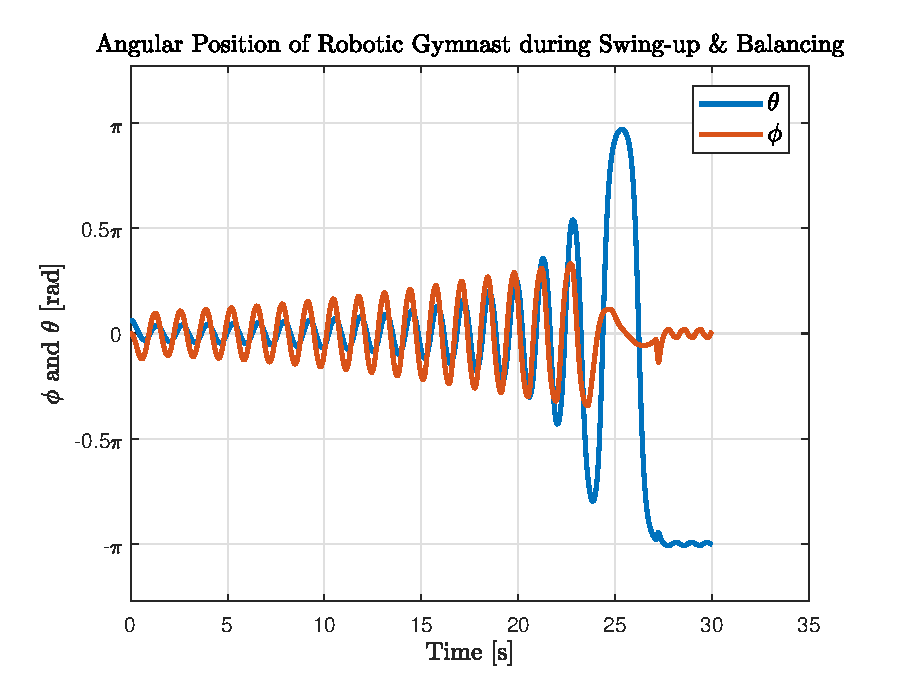
\includegraphics[scale=1]{./figs/swingup_balance}
	\caption{The Swing-Up \& Balancing of the Robotic Gymnast}
	\label{fig:swingup_balance}
\end{figure}